\begin{esercizio}
   A particle of mass $m$ is in a potential well given by
   \begin{equation*}
      V(x)=
      \begin{cases}
         +\infty & \text{for } x<0\\
         0 & \text{for } x<0<\frac{L}{2}\\
         V_0 & \text{for } \frac{L}{2}<x<L\\
         +\infty & \text{for } x>L\\
      \end{cases}
   \end{equation*}
   \begin{enumerate}[label=\alph*), leftmargin=0.6cm]
      \item Use perturbation theory to calculate the energy of the ground state $E_1^{(1)}$.
      \item For $m=1 \; \rm GeV$ and $L=2 \; \rm fm$ what is the value of $V_0$ to have $V_0=0.2E_1^{(1)}$?
      \item Under the condition in b), ($V_0 \ll E$), calculate the ground state energy with the WKB approximation.
      \item How the result in c) compares to the result in a)? (Explain)
   \end{enumerate}
\end{esercizio}
\begin{soluzione}
   Svolgiamo il punto a). Per prima cosa rappresentiamo il potenziale:

   \begin{figure}[H]
      \centering
      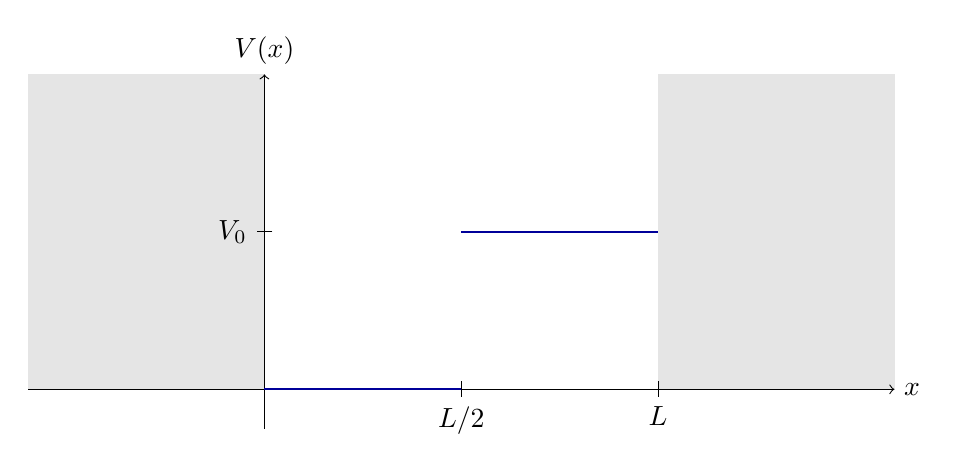
\begin{tikzpicture}
         \filldraw[gray!20!] (0,0) -- (0,4) -- (-3,4) -- (-3,0) -- cycle;
         \filldraw[gray!20!] (5,0) -- (5,4) -- (8,4) -- (8,0) -- cycle;
         \draw[->] (0,-0.5) -- (0,4) node[above] {$V(x)$};
         \draw[->] (-3,0) -- (8,0) node[right] {$x$};
         \draw[thick,blue!60!black] (0,0) -- (2.5,0);
         \draw[thick,blue!60!black] (2.5,2) -- (5,2);
         \draw (2.5,0.1) -- (2.5,-0.1) node[below] {$L/2$};
         \draw (5,0.1) -- (5,-0.1) node[below] {$L$};
         \draw (0.1,2) -- (-0.1,2) node[left] {$V_0$};
      \end{tikzpicture}
   \end{figure}

   Siamo ancora nell'ambito della teoria perturbativa, quindi dobbiamo identificare la correzione al potenziale imperturbato. Quest'ultimo è quello della buca quadra, dato da
   
   \begin{equation*}
      V_{\rm box}=
      \begin{cases}
         0 & \text{per } 0<x<L\\
         \infty & \text{altrimenti}\\
      \end{cases}
   \end{equation*}

   Le funzioni d'onda degli stati imperturbati sono date da
   
   \begin{equation*}
      \psi_n^{(0)}(x)
      =\sqrt{\frac{2}{L}} \sin{\qty( \frac{n \pi}{L} x)}
      \qq{,}
      n=1,2,\ldots
   \end{equation*}

   mentre le energie associate da

   \begin{equation*}
      E_n^{(0)}
      =\frac{\hbar^2 \pi^2 n^2}{2mL^2}
      \qq{,}
      n=1,2,\ldots
   \end{equation*}

   Riscriviamo quindi il potenziale $V$ come il potenziale $V_{\rm box}$ della buca quadra più un termine perturbativo $V'$. In particolare, quest'ultimo può essere scritto come
   
   \begin{equation*}
      \textstyle V'
      =V_0 \vartheta\qty(x - \frac{L}{2}) \vartheta (L - x)
   \end{equation*}
   
   dove le funzioni theta di Heaviside così fatte ci dicono che $V'$ contribuisce con un termine $V_0$ soltanto nella regione per $L/2<x<L$.
   
   A questo punto calcoliamo l'energia al primo ordine per il ground state. Per la teoria perturbativa indipendente dal tempo al primo ordine si ha che $E_1^{(1)}=E_1^{(0)} + \delta E_1^{(1)}$, dove la correzione al primo ordine $\delta E_1^{(1)}$ è data dall'elemento di matrice della perturbazione rispetto al ground state imperturbato del sistema:
   
   \begin{equation*}
      \delta E_1^{(1)}
      =\mel*{1^{(0)}}{V'(x)}{1^{(0)}}
      =\int_{-\infty}^{+\infty} \dd{x} \psi_1^*(x) V'(x) \psi_1(x)
   \end{equation*}

   Una volta che esplicitiamo $V(x)$, l'integrale risulta avere contributo non nullo soltanto nella regione per $L/2<x<L$, per cui
   \begin{equation*}
      \delta E_1^{(1)}
      =V_0 \int_{L/2}^{L} \dd{x} \frac{2}{L} \sin^2{ \qty( \frac{\pi x}{L} ) }
      =\frac{V_0}{L} \int_{L/2}^{L} \dd{x} \qty[ 1 - \cos{ \qty( \frac{2\pi x}{L} ) } ]
   \end{equation*}

   avendo usato la relazione trigonometrica $2 \sin^2{\alpha}=1 - \cos{(2\alpha)}$ nell'ultimo passaggio.

   Se adesso operiamo il cambiamento di variabile

   \begin{equation*}
      z=\frac{2\pi x}{L}
      \implies
      x=\frac{L z}{2\pi}
      \qq{,}
      \dd{x}=\frac{L \dd{z}}{2\pi}
   \end{equation*}

   Possiamo riscrivere l'integrale come

   \begin{equation*}
      \frac{V_0}{L} \int_{L/2}^{L} \dd{x} \qty[ 1 - \cos{ \qty( \frac{2\pi x}{L} ) } ]
      =\frac{V_0}{2\pi} \int_{\pi}^{2\pi} \dd{z} ( 1 - \cos{z} )
      =\frac{V_0}{2}
   \end{equation*}

   Abbiamo quindi trovato che la correzione al primo ordine al ground state imperturbato è pari a metà del potenziale. Il livello di energia corretto risulta dunque essere

   \begin{equation*}
      E_1^{(1)}
      =\frac{\hbar^2 \pi^2}{2mL^2} + \frac{V_0}{2}
   \end{equation*}
   
   Passiamo al punto b). Cerchiamo, fissati i valori forniti dal testo per la massa e per la larghezza della buca, il valore che deve avere $V_0$ per essere uguale a $0.2E_1^{(1)}$. Tale condizione può essere scritta come

   \begin{equation*}
      E_1^{(1)}=5V_0
      \iff
      \frac{\hbar^2 \pi^2}{2mL^2} + \frac{V_0}{2}=5V_0
      \implies
      V_0=\frac{\hbar^2 \pi^2}{9 m L^2}
   \end{equation*}

   Se in tale espressione estrapoliamo l'espressione dell'energia del ground state imperturbato possiamo scrivere ancora:

   \begin{equation*}
      V_0=\frac{\hbar^2 \pi^2}{9 m L^2}
      =\frac{2}{9} E_1^{(0)}
      \simeq 0.22 E_1^{(0)}
   \end{equation*}

   Da quest'ultima espressione deduciamo che $V_0 \sim 20\%E_1^{(0)}$ e che $\delta E_1^{(1)} \sim 10\%E_1^{(1)}$.

   A questo punto ricaviamo il valore di $V_0$ sostituendo i valori numerici. Cerchiamo di far spuntare quantità note moltiplicando e dividendo per $c^2$, in modo che al denominatore abbiamo la massa della particella che è data dal testo e al numeratore abbiamo la quantità $\hbar c$, che in questo caso conviene esprimere come $0.2 \; \rm GeV \, fm$:

   \begin{equation*}
      V_0
      =\frac{(\hbar c)^2 \pi^2}{9 (mc^2) L^2}
      =\rm \frac{4 \cdot 10^{-2} \; GeV^2\,fm^2 \cdot 10}{9 \cdot 1 \; GeV \cdot 4 \; fm^2}
      =\frac{1}{90} \; GeV
      \approx 11 \; MeV
   \end{equation*}

   Passiamo ora al quesito c). Nella condizione $V_0 \ll E$ (in cui siamo perché $V_0 \sim 20\% E$, dobbiamo calcolare l'energia dello stato fondamentale con l'approssimazione WKB.
   
   In questo caso ci troviamo davanti ad una buca con due pareti verticali, quindi la condizione per ottenere i livelli di energie approssimati è
   
   \begin{equation*}
      \int_{x_1}^{x_2} p(x) \dd{x}=n\pi\hbar
      \qq{,}
      n=1,2,\ldots
   \end{equation*}

   Nel problema in esame i turning points $x_1$ e $x_2$ sono $x_1=0$ e $x_2=L$. Sostituendo poi l'espressione del potenziale otteniamo
   
   \begin{gather*}
      \int_{0}^{L} p(x) \dd{x}
      =\int_{0}^{L} \sqrt{2m \bigl[ E - V(x) \bigr]} \dd{x}
      =\int_{0}^{L/2} \sqrt{2mE} \dd{x} + \int_{L/2}^{L} \sqrt{2m(E - V_0)} \dd{x}
      =\\
      =\sqrt{2mE} \frac{L}{2} + \sqrt{2m(E - V_0)} \frac{L}{2}
      =\sqrt{2m} \frac{L}{2} \qty( \sqrt{E} + \sqrt{E - V_0} )
      =n \pi \hbar
   \end{gather*}

   In particolare l'ultima uguaglianza può essere riscritta come

   \begin{equation*}
      \sqrt{E} + \sqrt{E - V_0}
      =\frac{2 n \pi \hbar}{\sqrt{2m} L}
   \end{equation*}

   A questo punto eleviamo entrambi i membri al quadrato:

   \begin{equation*}
      E + E - V_0 + 2\sqrt{E(E - V_0)}
      =\frac{4 n^2 \pi^2 \hbar^2}{2 m L^2}
      =4 E_n^{(0)}
   \end{equation*}

   A partire da tale relazione dobbiamo ricavare $E$. Per fare ciò isoliamo la radice al primo membro e poi eleviamo al quadrato:

   \begin{gather*}
      2\sqrt{E(E - V_0)}
      =4 E_n^{(0)} - 2E + V_0
      \\
      \implies
      4E(E - V_0)
      =16 \bigl( E_n^{(0)} \bigr)^2 + 4E^2 + V_0^2 - 16 E E_n^{(0)} - 4EV_0 + 8 V_0 E_n^{(0)}
      \\
      \implies
      16 \bigl( E_n^{(0)} \bigr)^2 + V_0^2 - 16 E E_n^{(0)} + 8 V_0 E_n^{(0)}=0
   \end{gather*}

   da cui infine si ottiene

   \begin{equation*}
      E=E_n^{(0)} + \frac{V_0}{2} + \frac{V_0^2}{16 E_n^{(0)}}
   \end{equation*}

   Notiamo che tale espressione è data dal risultato ottenuto con la teoria perturbativa più un termine aggiuntivo $\frac{V_0^2}{16 E_n^{(0)}}$. Se però ora sfruttiamo la condizione $V_0 \ll E$ fornita dal testo, tale energia si riduce semplicemente a

   \begin{equation*}
      E_n^{(0)} + \frac{V_0}{2}
   \end{equation*}

   Che è l'espressione che si ottiene con la teoria perturbativa.
   
   Svolgiamo infine il punto d). Facciamo un confronto utilizzando i valori numerici ottenuti prima. Riscriviamo l'espressione dei livelli energetici ottenuti per la WKB nel caso $n=1$ come
   
   \begin{equation*}
      E=E_1^{(0)} + \frac{V_0}{2} \qty( 1 + \frac{V_0}{8 E_1^{(0)}} )
   \end{equation*}

   Utilizzando i valori $V_0=1.1 \cdot 10^{-2} \; \rm GeV$, $E_1^{(0)}=5V_0=5 \cdot 10^{-2} \; \rm GeV$, si trova che
   
   \begin{equation*}
      \frac{V_0}{8 E_1^{(0)}} \approx 0.03 \ll 1
   \end{equation*}
   
   Possiamo allora effettivamente dire che, per i valori trovati nel punto b), siamo nel caso in cui tale termine risulta trascurabile e pertanto il risultato della WKB coincide con quello della teoria perturbativa.
\end{soluzione}

\newpage
\setcounter{equation}{0}

\begin{esercizio}
   An electron is in a potential given by
   \begin{equation*}
      V(x)=
      \begin{dcases}
         \infty & \text{for } x<0\\
         0 & \text{for } 0<x<\frac{L}{2}\\
         V_0 \qty( \frac{2x}{L} - 1 ) & \text{for } \frac{L}{2}<x<L\\
         \infty & \text{for } x>L\\
      \end{dcases}
   \end{equation*}
   \begin{enumerate}[label=\alph*), leftmargin=0.6cm]
      \item Use perturbation theory to calculate the energy\footnotemark\;of the ground state.
      \item What is the condition on $V_0$ to have perturbation theory valid?
      \item Put $V(x)=0$ for $x>L$ and $E<V_0$. Use WKB to calculate the penetrability of the barrier for $V_0=4 \; \rm MeV$, $L=10 \; \rm fm$ and $E=V_0/2$.
   \end{enumerate}
\end{esercizio}
\begin{soluzione}
   \footnotetext{Quando nel testo non è specificato, si intende fin al primo ordine.}

   Per prima cosa riportiamo in un grafico l'andamento del potenziale:

   \begin{figure}[H]
      \centering
      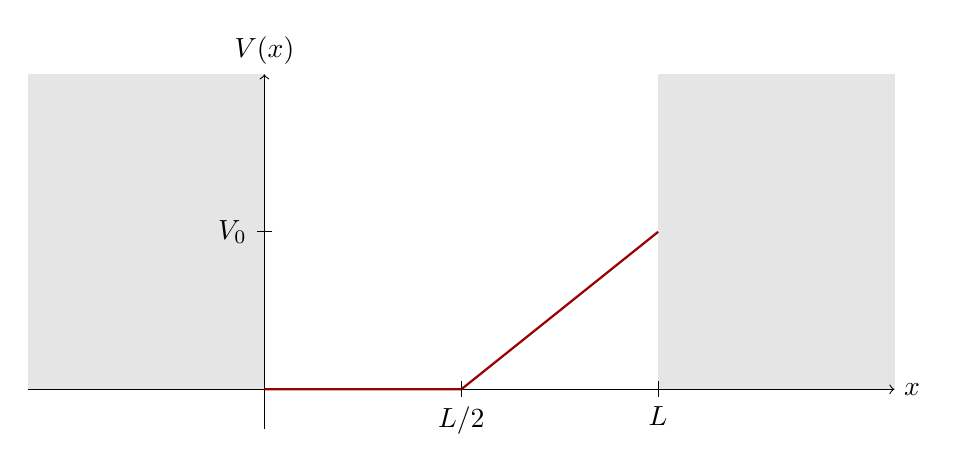
\begin{tikzpicture}
         \filldraw[gray!20!] (0,0) -- (0,4) -- (-3,4) -- (-3,0) -- cycle;
         \filldraw[gray!20!] (5,0) -- (5,4) -- (8,4) -- (8,0) -- cycle;
         \draw[->] (0,-0.5) -- (0,4) node[above] {$V(x)$};
         \draw[->] (-3,0) -- (8,0) node[right] {$x$};
         \draw[thick,red!60!black!] (0,0) -- (2.5,0) -- (5,2);
         \draw (2.5,0.1) -- (2.5,-0.1) node[below] {$L/2$};
         \draw (5,0.1) -- (5,-0.1) node[below] {$L$};
         \draw (0.1,2) -- (-0.1,2) node[left] {$V_0$};
      \end{tikzpicture}
   \end{figure}
   
   Svolgiamo il punto a). La correzione al primo ordine all'energia del ground state è data da
   
   \begin{gather*}
      \delta E_1^{(1)}
      =\mel*{\psi_1^{(0)}}{V'}{\psi_1^{(0)}}
      =\int_{L/2}^{L} \dd{x} V_0 \qty( \frac{2x}{L} - 1 ) \bigl| \psi_1^{(0)} \bigr|^2
      =\int_{L/2}^{L} \dd{x} V_0 \qty( \frac{2x}{L} - 1 ) \frac{2}{L} \sin^2{ \qty( \frac{\pi x}{L} ) }=
      \\
      =\frac{V_0}{L} \qty[ \int_{L/2}^{L} \dd{x} \qty( \frac{2x}{L} - 1 ) - \int_{L/2}^{L} \dd{x} \qty( \frac{2x}{L} - 1 ) \cos{\qty( \frac{2\pi x}{L} )}]
   \end{gather*}
   dove abbiamo sfruttato la relazione trigonometrica $2 \sin^2{\alpha}=1 - \cos{(2\alpha)}$ nell'ultimo passaggio.

   Calcoliamo adesso ciascun integrale: per il primo si ha banalmente

   \begin{equation*}
      \int_{L/2}^{L} \dd{x} \qty( \frac{2x}{L} - 1 )
      =\qty[ \frac{x^2}{L} - x]_{L/2}^{L}
      =L - L - \frac{L}{4} + \frac{L}{2}
      =\frac{L}{4}
   \end{equation*}

   Per quanto riguarda il secondo integrale, esso si può ulteriormente spezzare in due integrali:

   \begin{equation*}
      \int_{L/2}^{L} \dd{x} \qty( \frac{2x}{L} - 1 ) \cos{\qty( \frac{2\pi x}{L} )}
      =\int_{L/2}^{L} \dd{x} \frac{2x}{L} \cos{\qty( \frac{2\pi x}{L} )} - \int_{L/2}^{L} \dd{x} \cos{\qty( \frac{2\pi x}{L} )}
   \end{equation*}

   i quali, ponendo

   \begin{equation*}
      y=\frac{2\pi x}{L}
      \implies
      \dd{y}=\frac{2\pi \dd{x}}{L}
   \end{equation*}

   Possono esse riscritti come

   \begin{equation*}
      \frac{L}{2\pi^2} \int_{\pi}^{2\pi} \dd{y} y \cos{y} - \frac{L}{2\pi} \int_{\pi}^{2\pi} \dd{y} \cos{y}
   \end{equation*}

   Per il secondo integrale otteniamo subito che
   
   \begin{equation*}
      \frac{L}{2\pi} \int_{\pi}^{2\pi} \dd{y} \cos{y}
      =\frac{L}{2\pi} \qty[ \sin{y} ]_{\pi}^{2\pi}
      =0
   \end{equation*}

   Il primo invece va risolto per parti: ponendo $f=y$ e $g=\cos{y}$, si ha

   \begin{equation*}
      \frac{L}{2\pi^2} \int_{\pi}^{2\pi} y \cos{y} \dd{y}
      =\frac{L}{2\pi^2} \qty{ \bigl[ y \sin{y} \bigr]_{\pi}^{2\pi} - \int_{\pi}^{2\pi} \sin{y} \dd{y} }
      =\frac{L}{2\pi^2} \bigl[ \cos{y} \bigr]_{\pi}^{2\pi}
      =\frac{L}{\pi^2}
   \end{equation*}

   Mettendo insieme i vari contributi troviamo che

   \begin{equation*}
      \delta E_1^{(1)}
      =\frac{V_0}{L} \qty( \frac{L}{4} - \frac{L}{\pi^2} )
      =V_0\qty( \frac{1}{4} - \frac{1}{\pi^2} )
   \end{equation*}

   e pertanto l'energia del ground state corretta al primo ordine risulta essere

   \begin{equation*}
      E_1^{(1)}
      =E_1^{(0)} + \delta E_1^{(1)}
      =\frac{\hbar^2 \pi^2}{2 m L^2} + V_0\qty( \frac{1}{4} - \frac{1}{\pi^2} )
   \end{equation*}

   Passiamo al punto b). Ricordiamo che la condizione affinché la teoria perturbativa sia valida è che il rapporto tra la correzione di energia e la differenza di energia tra lo stato imperturbato e quello più vicino deve essere molto minore di 1; in particolare per il ground state si deve avere
   
   \begin{equation*}
      \qty| \frac{\delta E_1^{(1)}}{E_1^{(0)} - E_2^{(0)}} | \ll 1
   \end{equation*}

   Esplicitando quanto trovato, tale condizione si riscrive come

   \begin{equation*}
      \qty| \frac{V_0\qty( \frac{1}{4} - \frac{1}{\pi^2} )}{-3 \frac{\hbar^2 \pi^2}{2 m L^2}} |
      =\frac{mL^2 V_0 (\pi^2 - 4)}{6\hbar^2}
      \ll 1
   \end{equation*}

   da cui si ricava che la condizione per $V_0$ è

   \begin{equation*}
      V_0 \ll \frac{6\hbar^2}{m L^2 (\pi^2 - 4)}
   \end{equation*}
   
   Svolgiamo ora il punto c). Adesso il potenziale cambia e diventa nullo nella regione per $xL$, dunque graficamente adesso la situazione è la seguente:
   
   \begin{figure}[H]
      \centering
      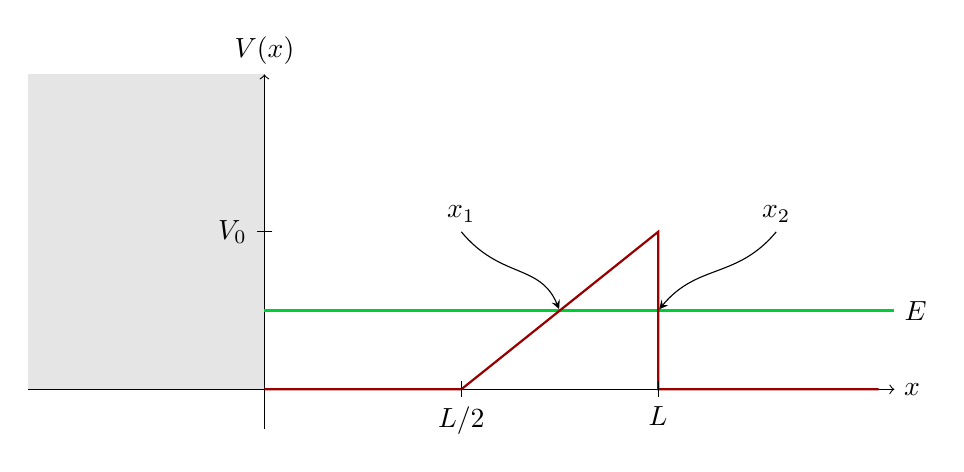
\begin{tikzpicture}
         \filldraw[gray!20!] (0,0) -- (0,4) -- (-3,4) -- (-3,0) -- cycle;
         \draw[->] (0,-0.5) -- (0,4) node[above] {$V(x)$};
         \draw[->] (-3,0) -- (8,0) node[right] {$x$};
         \draw[thick,green!60!teal!] (0,1) -- (8,1) node[right,black] {$E$};
         \draw[thick,red!60!black!] (0,0) -- (2.5,0) -- (5,2) -- (5,0) -- (7.8,0);
         \draw (2.5,0.1) -- (2.5,-0.1) node[below] {$L/2$};
         \draw (5,0.1) -- (5,-0.1) node[below] {$L$};
         \draw (0.1,2) -- (-0.1,2) node[left] {$V_0$};
         \draw[-stealth,shorten >= 0.6pt] (6.5,2) node[above] {$x_2$} .. controls (6,1.4) and (5.5,1.6) .. (5,1);
         \draw[-stealth,shorten >= 0.6pt] (2.5,2) node[above] {$x_1$} .. controls (3,1.4) and (3.5,1.6) .. (3.75,1);
      \end{tikzpicture}
   \end{figure}

   In questo caso dobbiamo usare la WKB per calcolare la penetrabilità della barriera (quindi siamo nel caso in cui $E<V_0$), che è data da

   \begin{equation*}
      T
      \approx \exp{ -\frac{2}{\hbar} \int_{x_1}^{x_2} \dd{x} \sqrt{ 2m \bigl[ V(x) - E \bigr] } }
   \end{equation*}

   dove $x_1$ e $x_2$ sono i turning points. La prima cosa da fare è proprio individuare questi ultimi. Si intuisce facilmente che $x_2=L$, mentre per $x_1$ dobbiamo uguagliare energia e potenziale:

   \begin{equation*}
      E=V_0\qty( \frac{2x_1}{L} - 1 )
      \implies
      x_1
      =\frac{L}{2}\qty( \frac{E}{V_0} + 1 )
   \end{equation*}

   Se adesso applichiamo la condizione fornita dal testo per cui $E=V_0/2$, troviamo che

   \begin{equation*}
      x_1
      =\frac{L}{2}\qty( \frac{V_0}{2V_0} + 1 )
      =\frac{3}{4} L
   \end{equation*}

   Possiamo quindi calcolare

   \begin{gather*}
      T
      =\exp{ -\frac{2}{\hbar} \int_{x_1}^{x_2} \dd{x} \sqrt{ 2m \qty[ V_0\qty( \frac{2x}{L} - 1 ) - E ] } }
   \end{gather*}

   Introduciamo la variabile

   \begin{equation*}
      z=2m \qty[ V_0\qty( \frac{2x}{L} - 1 ) - E ]
      \implies
      \dd{z}=\frac{4mV_0}{L} \dd{x}
   \end{equation*}

   da cui segue che

   \begin{gather*}
      z_1
      =2m \qty[ V_0\qty( \frac{2x_1}{L} - 1 ) - E ]
      =2m \qty{ V_0\qty[ \frac{2}{L} \frac{L}{2}\qty( \frac{E}{V_0} + 1 ) - 1 ] - E }
      =0
      \\[0.1cm]
      z_2
      =2m \qty[ V_0\qty( \frac{2x_2}{L} - 1 ) - E ]
      =2m (V_0 - E)
   \end{gather*}

   Usando tale cambio di variabile, l'integrale si può riscrivere come

   \begin{equation*}
      T
      \approx
      \exp{ -\frac{2L}{4 m V_0 \hbar} \int_{0}^{2m(V_0 - E)} \dd{z} \sqrt{z} }
      =\exp{ -\frac{L}{3 m \hbar V_0} \bigl[ 2m(V_0 - E) \bigr]^{\frac{3}{2}} }
   \end{equation*}

   Passiamo infine il punto d). Per prima cosa moltiplichiamo e dividiamo per $c^3$ in modo da far spuntare quantità note, in particolare $\hbar c$ e $mc^2$. Sostituendo poi i valori numerici forniti dal testo, si ha

   \begin{gather*}
      T
      \approx \exp{ - \frac{L}{3 mc^2 \hbar c V_0} \bigl[ 2 mc^2 (V_0 - E) \bigr]^{\frac{3}{2}} }
      =\\
      =\rm \exp{ - \frac{10 \; fm}{0.5 \; MeV \cdot 2 \cdot 10^2 \; MeV \, fm \cdot 3 \cdot 4 \; MeV} \bigl[ 2 \cdot 0.5 \; MeV (4 - 2) MeV \bigr]^{\frac{3}{2}} }
      =\\
      =\exp{ -\frac{1}{120} 2^{\frac{3}{2}} }
      =\exp{-\frac{\sqrt{2}}{60}}
      =0.98
   \end{gather*}
\end{soluzione}

\newpage
\setcounter{equation}{0}

\begin{esercizio}
   A biatomic molecule is composed by two identical nuclei. The potential of the system is
   \begin{equation*}
      U_{\rm tot}=U\qty( \qty| \vb{r} + \frac{\vb{a}}{2} | ) + U\qty( \qty| \vb{r} - \frac{\vb{a}}{2} | )
   \end{equation*}
   The two nuclei have the centres at a distance $|\vb{a}|$ and
   \begin{equation*}
      U(|\vb{r}|)=
      \begin{cases}
         -V_0 & \text{for } 0<r<r_0\\
         0 & \text{elsewhere}
      \end{cases}
   \end{equation*}
   \begin{enumerate}[label=\alph*), leftmargin=0.6cm]
      \item Calculate the differential cross section in first order Born approximation for a particle of mass $m$ in terms of the exchanged momentum $\vb{q}$.
      \item What is the differential cross section in the limit $|\vb{q}| \ll |\vb{a}|^{-1}$? Juustify your answer.
   \end{enumerate}
   Hint: evaluate first the scattering amplitude for $U(\vb{r})=-V_0$ and then use an appropriate substitution.
\end{esercizio}
\begin{soluzione}
   Schematizziamo la situazione:
   \begin{figure}[H]
      \centering
      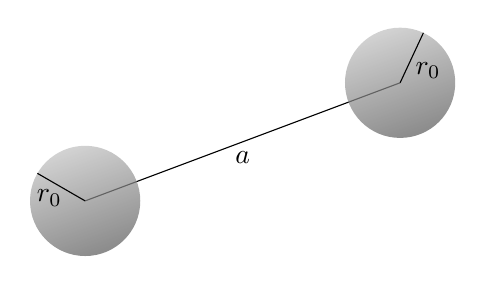
\begin{tikzpicture}
         \draw (0,0) -- (4,1.5) node[midway,below] {$a$};
         \shade[top color=gray!50,bottom color=gray!70!black,shading angle=20,opacity=0.7] (0,0) circle (0.7cm);
         \shade[top color=gray!50,bottom color=gray!70!black,shading angle=20,opacity=0.7] (4,1.5) circle (0.7cm);
         \draw[rotate=150] (0,0) -- (0.7,0) node[near end,below] {$r_0$};
         \draw[shift={(4,1.5)},rotate=65] (0,0) -- ++(0.7,0) node[near start,right] {$r_0$};
      \end{tikzpicture}
   \end{figure}
   In questo problema abbiamo 2 nuclei distanti $a$ tra loro, ognuno dei quali ha potenziale che approssimiamo con un potenziale costante entro un range $r_0$. Il quesito a) ci chiede di calcolare la sezione d'urto differenziale in approssimazione di Born al primo ordine in funzione del momento scambiato $\vb{q}$. Per prima cosa allora calcoliamo l'ampiezza di scattering, che nell'approssimazione di Born è data da\footnote{Da notare che nel termine $e^{-i \vb{q}}$ compare il segno meno perché abbiamo definito $\vb{q}$ come $\vb{k}'-\vb{k}$.}
   \begin{equation*}
      f^{\rm Born}(\vb{k},\vb{k}')
      =-\frac{m}{2\pi\hbar^2} \int \dd[3]{\vb{x}} e^{-i \vb{q} \vdot \vb{x}'} V(\vb{x}')
   \end{equation*}
   dove $V(\vb{x}')$ è la somma dei due potenziali. Poiché però se consideriamo insieme i due potenziali tale integrale risulta di difficile risoluzione, analizziamo separatamente ciascuno dei due contributi. Consideriamo prima il nucleo di sinistra: avremo che il suo contributo è\footnote{Per coerenza nella notazione abbiamo ridefinito con $\vb{r}$ la variabile di integrazione.}
   \begin{equation*}
      \int \dd[3]{\vb{r}} e^{-i \vb{q} \vdot \vb{r}'} U\qty( \qty| \vb{r} + \frac{\vb{a}}{2} | )
   \end{equation*}
   Operiamo adesso il cambio di variabili $\vb{z}=\vb{r} + \frac{\vb{a}}{2}$, per cui l'integrale diventa
   \begin{equation*}
      \int \dd[3]{\vb{z}} e^{-i \vb{q} \vdot \vb{z}} e^{-i \vb{q} \vdot \frac{\vb{a}}{2}} U(|\vb{z}|)
   \end{equation*}
   Sfruttiamo ora il fatto che il potenziale è a simmetria sferica: ponendo $x=|\vb{z}|$, possiamo scrivere
   \begin{equation*}
      e^{i \vb{q} \vdot \frac{\vb{a}}{2}} 2\pi \int_{0}^{\infty} \dd{x} x^2 U(x) \int_{-1}^{1} \dd{(\cos{\vartheta})} e^{-i q x \cos{\vartheta}}
   \end{equation*}
   dove il fattore $2\pi$ è dovuto all'integrazione rispetto a $\varphi$. Osserviamo che per la parte angolare si ha
   \begin{equation*}
      \int_{-1}^{1} \dd{(\cos{\vartheta})} e^{-i q x \cos{\vartheta}}
      = \frac{2 \sin{(q x)}}{q x}
   \end{equation*}
   e dunque l'integrale diventa
   \begin{equation*}
      \frac{4\pi}{q} e^{ i \vb{q} \vdot \frac{\vb{a}}{2} } \int_{0}^{\infty} \dd{x} x U(x) \sin{(qx)}
   \end{equation*}
   Poiché però il potenziale è nullo al di fuori di $r_0$, possiamo estendere l'integrazione fino a $r_0$ (dove in particolare è uguale a $-V_0$) e ottenere
   \begin{equation*}
      -V_0 \frac{4\pi}{q} e^{i \vb{q} \vdot \frac{\vb{a}}{2} } \int_{0}^{r_0} \dd{x} x \sin{(qx)}
      =-\frac{4\pi V_0}{q^3} e^{ i \vb{q} \vdot \frac{\vb{a}}{2} } \bigl[ \sin{(qr_0)} - qr_0\cos{(qr_0)} \bigr]
   \end{equation*}
   avendo integrato per parti.\\
   In maniera analoga ma operando stavolta la sostituzione $\vb{z}=\vb{r} - \frac{\vb{a}}{2}$, si ottiene
   \begin{equation*}
      \int \dd[3]{\vb{r}} e^{-i \vb{q} \vdot \vb{r}'} U\qty( \qty| \vb{r} + \frac{\vb{a}}{2} | )
      =-\frac{4\pi V_0}{q^3} e^{ -i \vb{q} \vdot \frac{\vb{a}}{2} } \bigl[ \sin{(qr_0)} - qr_0\cos{(qr_0)} \bigr]
   \end{equation*}
   In definitiva l'ampiezza di scattering risulta essere
   \begin{equation*}
      \begin{split}
         f^{\rm Born}(\vb{k},\vb{k}')
         & =-\frac{2 m V_0}{\hbar^2 q^3} \qty( e^{ i \vb{q} \vdot \frac{\vb{a}}{2} } + e^{ -i \vb{q} \vdot \frac{\vb{a}}{2} } ) \bigl[ \sin{(qr_0)} - qr_0\cos{(qr_0)} \bigr]
         \\[0.1cm]
         & =-\frac{4 m V_0}{\hbar^2 q^3} \cos{ \qty( \frac{\vb{q} \vdot \vb{a}}{2} ) } \bigl[ \sin{(qr_0)} - qr_0\cos{(qr_0)} \bigr]
      \end{split}
   \end{equation*}
   e dunque la sezione d'urto differenziale sarà
   \begin{equation}
      \dv{\sigma}{\Omega}
      =\bigl| f^{\rm Born}(\vb{k},\vb{k}') \bigr|^2
      =\frac{16 m^2 V_0^2}{\hbar^4 q^6} \cos^2{ \qty( \frac{\vb{q} \vdot \vb{a}}{2} ) } \bigl[ \sin{(qr_0)} - qr_0\cos{(qr_0)} \bigr]^2
      \label{eq:diff_cross_section_molecola_biatomica}
   \end{equation}
   Passiamo al quesito b). La condizione $|\vb{q}| \ll |\vb{a}|^{-1}$ significa $|\vb{q}| |\vb{a}| \ll 1$, per cui è lecito fare l'approssimazione
   \begin{equation*}
      \cos{ \qty( \frac{\vb{q} \vdot \vb{a}}{2} ) } \simeq 1
   \end{equation*}
   Osserviamo inoltre che per un potenziale della forma di $U(\vb{r})$ avente profondità $-V_0$ la sezione d'urto differenziale è data da
   \begin{equation*}
      \qty( \dv{\sigma}{\Omega} )_0
      =\frac{4 m^2 V_0^2 r_0^2}{\hbar^4 q^4} \qty[ \frac{\sin{(qr_0)}}{qr_0} - \cos{(qr_0)} ]^2
   \end{equation*}
   Cerchiamo allora di ricondurre la \eqref{eq:diff_cross_section_molecola_biatomica} a tale forma. Si trova che
   \begin{equation*}
      \begin{split}
         \dv{\sigma}{\Omega}
         & =\frac{16 m^2 V_0^2}{\hbar^4 q^6} \bigl[ \sin{(qr_0)} - qr_0\cos{(qr_0)} \bigr]^2
           =4 \frac{4 m^2 V_0^2}{\hbar^4 q^6} (qr_0)^2 \qty[ \frac{\sin{(qr_0)}}{qr_0} - \cos{(qr_0)} ]^2
         \\[0.1cm]
         & =\frac{4 m^2 (2 V_0)^2 r_0^2}{\hbar^4 q^4} \qty[ \frac{\sin{(qr_0)}}{qr_0} - \cos{(qr_0)} ]^2
      \end{split}
   \end{equation*}
   che è la sezione d'urto di un potenziale della forma di $U(\vb{r})$ di profondità $-2V_0$. Quest'ultimo risultato ci dice che la sezione d'urto di due buche di profondità $-V_0$ e distanti $a$ tra loro è equivalente a quella di un sistema caratterizzato da un'unica buca avente ancora range $r_0$ ma profondità doppia\footnote{Un altro modo di vedere il problema è dire che la sezione d'urto del sistema è equivalente a quella di un'unica buca avente profondità $-V_0$ ma range $2r_0$.}. Ciò significa che, nella condizione $|\vb{q}| \ll |\vb{a}|^{-1}$ la particella non riesce a risolvere la doppia buca, cioè vede il sistema come se fosse un'unica buca di profondità doppia.
\end{soluzione}

\setcounter{equation}{0}